\subsection{Hybrid approach}
To create a hybrid solver we first assume that on average there are for each triangle pair distance computation only a few iterations that are required to arrive to a solution \ref{}. Based on empirical studies and tuning of the penalty parameter and the regularization variable, the majority of triangle pairs are solved within four iterations as shown in Figure {}. Secondly we set a user defined tolerance of error to the method to act as the switching point for the falling-back to brute force solver. If the number of fall backs does not overtake the number of penalty-based solutions then the method is a compromise between brute force and penalty both in terms of performance but also in terms of error of solution. 

\begin{figure}[htb]
  \begin{center}
    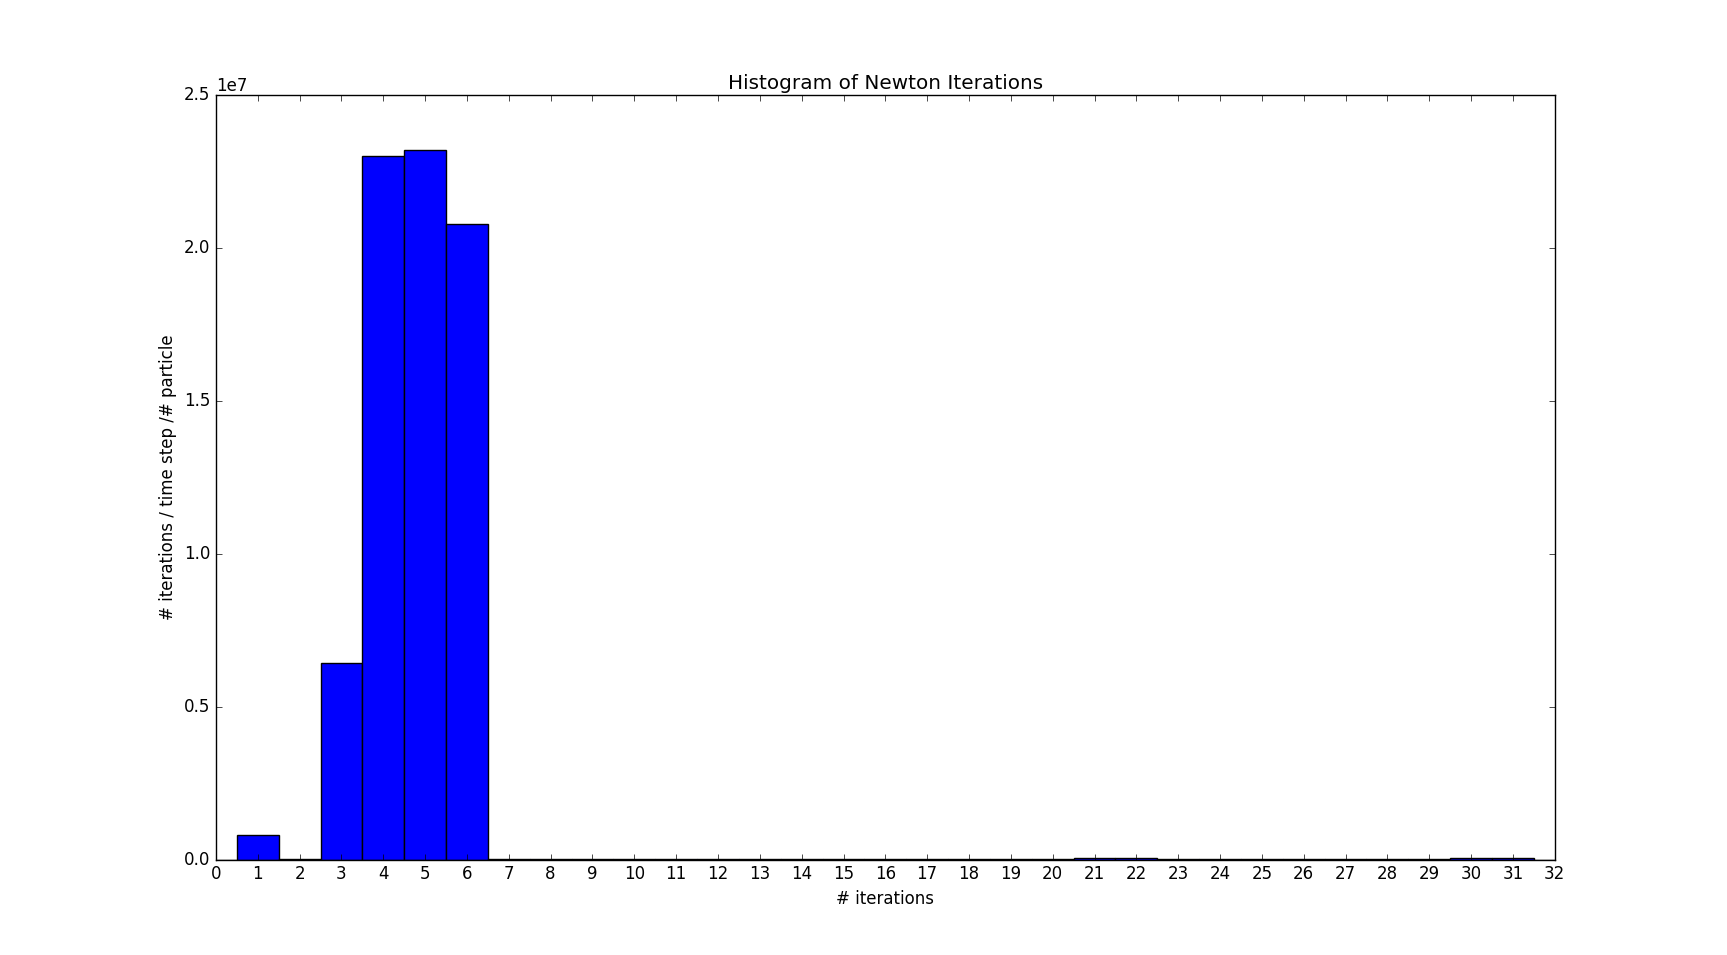
\includegraphics[width=1\textwidth]{experiments/random/penalty-stats/bar.png}
  \end{center}
  \caption{Histogram of number of iterations required by Newton Method for convergence on a sample of twenty four million triangle pair configurations.}
  \label{figure:newton_hist}
\end{figure}

There are two variants of hybrid method; the first is the hybrid-on-triangle-pairs and the second one is hybrid-on-triangle-batches. Both variants are developed to exploit the robustness of brute force while keeping the arithmetic intensity of the penalty method. The implementation of both methods takes into account the potential for shared memory scaling as well as data access continuity. In addition SIMD vectorised performance of the underlying methods and memory alignment are critical for the execution of both methods.

The first variant is hybrid-on-triangle-pairs where it divides the computational workload to be per each triangle pair. The hybrid-on-triangle-pairs method runs first the penalty solver on one triangle pair, if the solution is not within the user specified tolerance, we fall back to brute force to solve the problem naively. 

\begin{algorithm}
 \caption{Hybrid On Triangle Pairs} \label{algorithm:hybridTriangle}
 \begin{algorithmic}[1]

	\Function {hybridOnTrianglePairs(particleA, particleB, tolerance)}	
	
		\For {i = 0 to n particleA.triangles}
	
			\For {j = 0 to n particleB.triangles}
			
				\State {triangleError = penalty(particleA[i], particleB[j])}

				\If {triangleError > tolerance}

					\State {bruteForce(particleA[i], particleB[j])}
	
				\EndIf
	
			\EndFor
			
		\EndFor
		
		\Return {P, Q points on two triangles}
	
	\EndFunction
	
 \end{algorithmic}
\end{algorithm} 

The other variant is the hybrid-on-batches where it is hybrid per triangle batches. This method is checking the error less frequently than the previous variant and uses an error for the whole batch. As in the hybrid-on-triangle-pairs variant; we run then penalty method on one batch of triangles and then fall back to brute on the whole batch if the error tolerance is not satisfied. The batch size can be set by the user to be of any arbitrary size. For our application we set it to be the number of triangles of our non-spherical particles (tessellation size of 60~ triangles).    

\begin{algorithm}
 \caption{Hybrid On Triangle Batches} \label{algorithm:hybridBatches}
 \begin{algorithmic}[1]
	
	\Function {hybridOnTrianglePairs(particleA, particleB, tolerance)}	
	
		\For {i = 0 to n particleA.triangles}
	
			\For {j = 0 to n particleB.triangles (batchSize)}
					
				\State {batchError = penalty(particleA[i], particleB[j])}

			\EndFor
			
			\If {batchError > tolerance}
				
				\For {j = 0 to n particleB.triangles}
	
					\State {bruteForce(particleA[i], particleB[j])}

				\EndFor
	
			\EndIf
	
		\EndFor
	
		\Return {P, Q points on two triangles}	
	
	\EndFunction
	
 \end{algorithmic}
\end{algorithm} 

Both hybrid methods suffer by their nature by the granularity of the grain size whether that is singular size (triangle pair) or greater (batches of pairs).
The memory distribution of pairs of triangles that do not converge within the mean number of Newton iterations are not known a priori because the solution depends on the underlying geometry. Triangle pairs or triangle batches that do not converge within the set tolerance skew the overall error distribution margin, potentially creating the worse case scenario where the method becomes a worse than brute force solver with both penalty and brute force being executed in sequence. It is not possible to predict the sparsity/distribution of non-convergent triangle pairs/batches during run-time so the tolerance value, penalty, regularization parameters are vital. In our experiments those parameters are set based on empirical tuning and trial and error.

